\documentclass{beamer}

% xcolor and define colors -------------------------
\usepackage{xcolor}

% https://www.viget.com/articles/color-contrast/
\definecolor{purple}{HTML}{5601A4}
\definecolor{navy}{HTML}{0D3D56}
\definecolor{ruby}{HTML}{9a2515}
\definecolor{alice}{HTML}{107895}
\definecolor{daisy}{HTML}{EBC944}
\definecolor{coral}{HTML}{F26D21}
\definecolor{kelly}{HTML}{829356}
\definecolor{cranberry}{HTML}{E64173}
\definecolor{jet}{HTML}{131516}
\definecolor{asher}{HTML}{555F61}
\definecolor{slate}{HTML}{314F4F}

% Mixtape Sessions
\definecolor{picton-blue}{HTML}{00b7ff}
\definecolor{violet-red}{HTML}{ff3881}
\definecolor{sun}{HTML}{ffaf18}
\definecolor{electric-violet}{HTML}{871EFF}

\newcommand\pictonBlue[1]{{\color{picton-blue}#1}}
\newcommand\sun[1]{{\color{sun}#1}}
\newcommand\electricViolet[1]{{\color{electric-violet}#1}}
\newcommand\violetRed[1]{{\color{violet-red}#1}}

\newcommand\bgPictonBlue[1]{{\colorbox{picton-blue!20!white}{#1}}}
\newcommand\bgSun[1]{{\colorbox{sun!20!white}{#1}}}
\newcommand\bgElectricViolet[1]{{\colorbox{electric-violet!20!white}{#1}}}
\newcommand\bgVioletRed[1]{{\colorbox{violet-red!20!white}{#1}}}

\def\code#1{\texttt{#1}}

% Main theme colors
\definecolor{accent}{HTML}{00b7ff}
\definecolor{accent2}{HTML}{871EFF}
\definecolor{gray100}{HTML}{f3f4f6}
\definecolor{gray800}{HTML}{1F292D}


% Beamer Options -------------------------------------

% Background
\setbeamercolor{background canvas}{bg = white}

% Change text margins
\setbeamersize{text margin left = 15pt, text margin right = 15pt} 

% \alert
\setbeamercolor{alerted text}{fg = accent2}

% Frame title
\setbeamercolor{frametitle}{bg = white, fg = jet}
\setbeamercolor{framesubtitle}{bg = white, fg = accent}
\setbeamerfont{framesubtitle}{size = \small, shape = \itshape}

% Block
\setbeamercolor{block title}{fg = white, bg = accent2}
\setbeamercolor{block body}{fg = gray800, bg = gray100}

% Title page
\setbeamercolor{title}{fg = gray800}
\setbeamercolor{subtitle}{fg = accent}

%% Custom \maketitle and \titlepage
\setbeamertemplate{title page}
{
    %\begin{centering}
        \vspace{20mm}
        {\Large \usebeamerfont{title}\usebeamercolor[fg]{title}\inserttitle}\\
        {\large \itshape \usebeamerfont{subtitle}\usebeamercolor[fg]{subtitle}\insertsubtitle}\\ \vspace{10mm}
        {\insertauthor}\\
        {\color{asher}\small{\insertdate}}\\
    %\end{centering}
}

% Table of Contents
\setbeamercolor{section in toc}{fg = accent!70!jet}
\setbeamercolor{subsection in toc}{fg = jet}

% Button 
\setbeamercolor{button}{bg = accent}

% Remove navigation symbols
\setbeamertemplate{navigation symbols}{}

% Table and Figure captions
\setbeamercolor{caption}{fg=jet!70!white}
\setbeamercolor{caption name}{fg=jet}
\setbeamerfont{caption name}{shape = \itshape}

% Bullet points

%% Fix spacing between items
\let\olditemize=\itemize 
\let\endolditemize=\enditemize 
\renewenvironment{itemize}{\vspace{0.25em}\olditemize \itemsep0.25em}{\endolditemize}

%% Fix left-margins
\settowidth{\leftmargini}{\usebeamertemplate{itemize item}}
\addtolength{\leftmargini}{\labelsep}

%% enumerate item color
\setbeamercolor{enumerate item}{fg = accent}
\setbeamerfont{enumerate item}{size = \small}
\setbeamertemplate{enumerate item}{\insertenumlabel.}

%% itemize
\setbeamercolor{itemize item}{fg = accent!70!white}
\setbeamerfont{itemize item}{size = \small}
\setbeamertemplate{itemize item}[circle]

%% right arrow for subitems
\setbeamercolor{itemize subitem}{fg = accent!60!white}
\setbeamerfont{itemize subitem}{size = \small}
\setbeamertemplate{itemize subitem}{$\rightarrow$}

\setbeamertemplate{itemize subsubitem}[square]
\setbeamercolor{itemize subsubitem}{fg = jet}
\setbeamerfont{itemize subsubitem}{size = \small}








% Links ----------------------------------------------

\usepackage{hyperref}
\hypersetup{
  colorlinks = true,
  linkcolor = accent2,
  filecolor = accent2,
  urlcolor = accent2,
  citecolor = accent2,
}


% Line spacing --------------------------------------
\usepackage{setspace}
\setstretch{1.35}


% \begin{columns} -----------------------------------
\usepackage{multicol}


% Fonts ---------------------------------------------
% Beamer Option to use custom fonts
\usefonttheme{professionalfonts}

% \usepackage[utopia, smallerops, varg]{newtxmath}
% \usepackage{utopia}
\usepackage[sfdefault,light]{roboto}

% Small adjustments to text kerning
\usepackage{microtype}



% Remove annoying over-full box warnings -----------
\vfuzz2pt 
\hfuzz2pt


% Table of Contents with Sections
\setbeamerfont{myTOC}{series=\bfseries, size=\Large}
\AtBeginSection[]{
        \frame{
            \frametitle{Roadmap}
            \tableofcontents[current]   
        }
    }


% Tables -------------------------------------------
% Tables too big
% \begin{adjustbox}{width = 1.2\textwidth, center}
\usepackage{adjustbox}
\usepackage{array}
\usepackage{threeparttable, booktabs, adjustbox}
    
% Fix \input with tables
% \input fails when \\ is at end of external .tex file
\makeatletter
\let\input\@@input
\makeatother

% Tables too narrow
% \begin{tabularx}{\linewidth}{cols}
% col-types: X - center, L - left, R -right
% Relative scale: >{\hsize=.8\hsize}X/L/R
\usepackage{tabularx}
\newcolumntype{L}{>{\raggedright\arraybackslash}X}
\newcolumntype{R}{>{\raggedleft\arraybackslash}X}
\newcolumntype{C}{>{\centering\arraybackslash}X}

% Figures

% \imageframe{img_name} -----------------------------
% from https://github.com/mattjetwell/cousteau
\newcommand{\imageframe}[1]{%
    \begin{frame}[plain]
        \begin{tikzpicture}[remember picture, overlay]
            \node[at = (current page.center), xshift = 0cm] (cover) {%
                \includegraphics[keepaspectratio, width=\paperwidth, height=\paperheight]{#1}
            };
        \end{tikzpicture}
    \end{frame}%
}

% subfigures
\usepackage{subfigure}


% Highlight slide -----------------------------------
% \begin{transitionframe} Text \end{transitionframe}
% from paulgp's beamer tips
\newenvironment{transitionframe}{
    \setbeamercolor{background canvas}{bg=accent!40!black}
    \begin{frame}\color{accent!10!white}\LARGE\centering
}{
    \end{frame}
}


% Table Highlighting --------------------------------
% Create top-left and bottom-right markets in tabular cells with a unique matching id and these commands will outline those cells
\usepackage[beamer,customcolors]{hf-tikz}
\usetikzlibrary{calc}
\usetikzlibrary{fit,shapes.misc}

% To set the hypothesis highlighting boxes red.
\newcommand\marktopleft[1]{%
    \tikz[overlay,remember picture] 
        \node (marker-#1-a) at (0,1.5ex) {};%
}
\newcommand\markbottomright[1]{%
    \tikz[overlay,remember picture] 
        \node (marker-#1-b) at (0,0) {};%
    \tikz[accent!80!jet, ultra thick, overlay, remember picture, inner sep=4pt]
        \node[draw, rectangle, fit=(marker-#1-a.center) (marker-#1-b.center)] {};%
}


% DAGS ----------------------------------------------
\usepackage{tikz}
\usetikzlibrary{shapes,decorations,arrows,calc,arrows.meta,fit,positioning}
% Tikz settings optimized for causal graphs.
\tikzset{
    -Latex,auto,node distance =1 cm and 1 cm,semithick,
    state/.style ={ellipse, draw, minimum width = 0.7 cm},
    point/.style = {circle, draw, inner sep=0.04cm,fill,node contents={}},
    bidirected/.style={Latex-Latex,dashed},
    el/.style = {inner sep=2pt, align=left, sloped}
}


% Beamer tricks -------------------------------------
% Make \pause work in align environments
\makeatletter
\renewrobustcmd{\beamer@@pause}[1][]{%
  \unless\ifmeasuring@%
  \ifblank{#1}%
    {\stepcounter{beamerpauses}}%
    {\setcounter{beamerpauses}{#1}}%
  \onslide<\value{beamerpauses}->\relax%
  \fi%
}
\makeatother

\usepackage{breqn} % Breaks lines

\usepackage{amsmath}
\usepackage{mathtools}

\usepackage{pdfpages} % \includepdf

\usepackage{listings} % R code
\usepackage{verbatim} % verbatim

% Video stuff
\usepackage{media9}

% packages for bibs and cites
\usepackage{natbib}
\usepackage{har2nat}
\newcommand{\possessivecite}[1]{\citeauthor{#1}'s \citeyearpar{#1}}
\usepackage{breakcites}
\usepackage{alltt}

% Setup math operators
\DeclareMathOperator{\E}{E} \DeclareMathOperator{\tr}{tr} \DeclareMathOperator{\se}{se} \DeclareMathOperator{\I}{I} \DeclareMathOperator{\sign}{sign} \DeclareMathOperator{\supp}{supp} \DeclareMathOperator{\plim}{plim}
\DeclareMathOperator*{\dlim}{\mathnormal{d}\mkern2mu-lim}
\newcommand\independent{\protect\mathpalette{\protect\independenT}{\perp}}
   \def\independenT#1#2{\mathrel{\rlap{$#1#2$}\mkern2mu{#1#2}}}
\newcommand*\colvec[1]{\begin{pmatrix}#1\end{pmatrix}}

\newcommand{\myurlshort}[2]{\href{#1}{\textcolor{gray}{\textsf{#2}}}}


\begin{document}

\imageframe{./lecture_includes/mixtape_did_cover.png}


% ---- Content ----

\section{Diff-in-diff Checklist}

\subsection{Craigslist Example}

\begin{frame}{Checklist}

\begin{itemize}

\item We will be using this to go through steps of a checklist that has been presented in Roth, et. al. (2023) "What's Trending \dots"
\item I'll be explaining the checklist in the context of my project with Christine Durrance and Melanie Guldi looking at the effect of online dating on families
\item Empirical context will be Craigslist's Personals

\end{itemize}

\end{frame}


\begin{frame}{History of Online Dating}

\begin{figure}[ht]
    \centering
    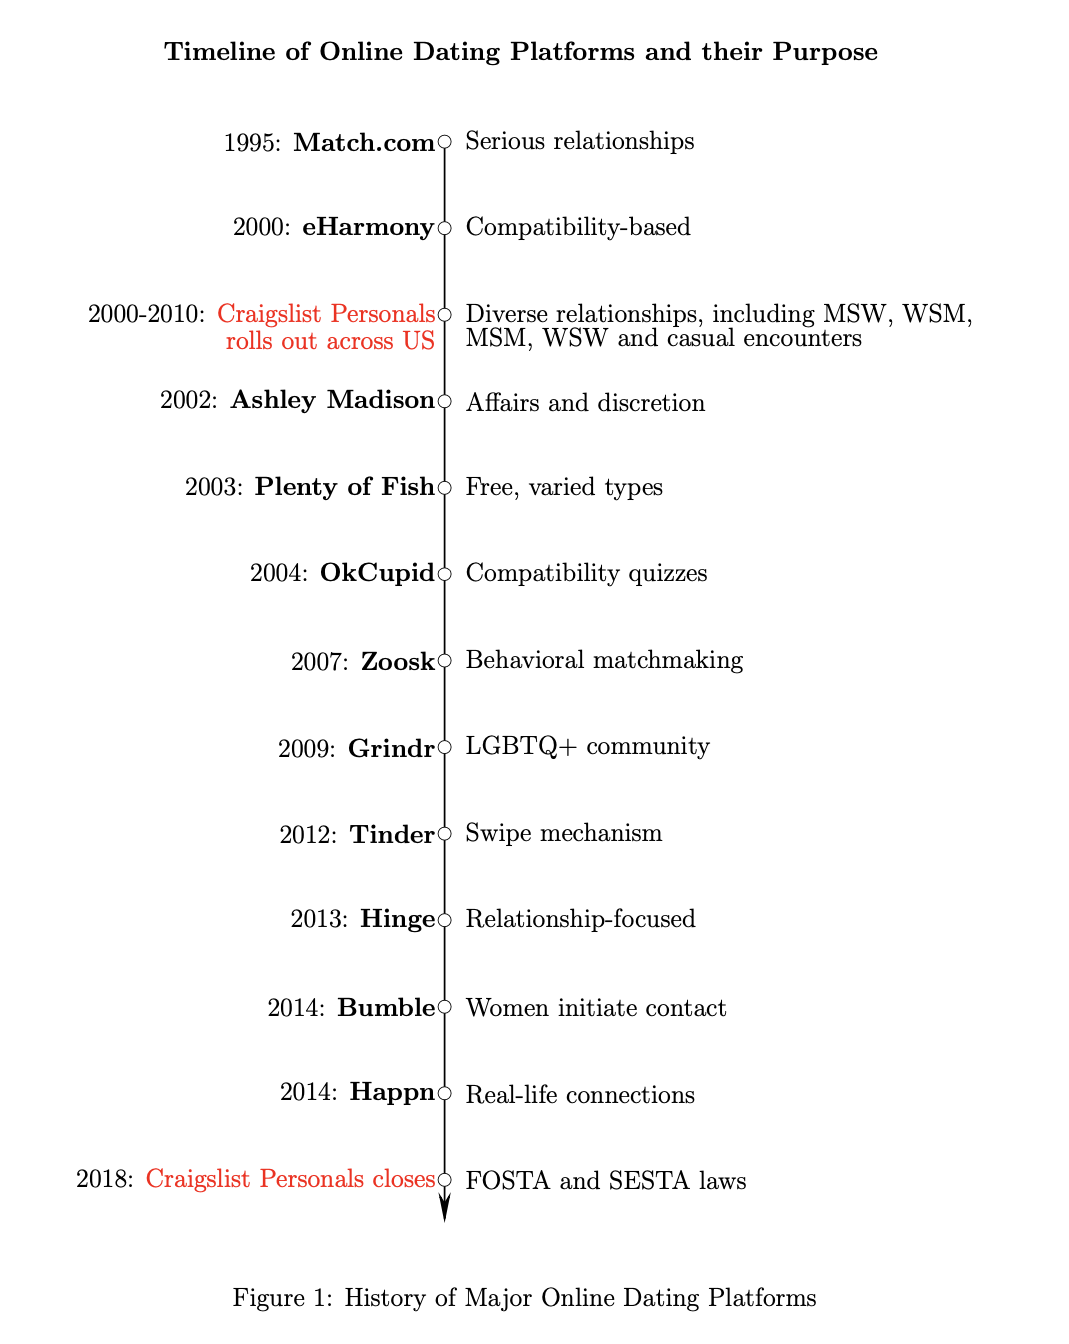
\includegraphics[width=\linewidth, height=0.8\textheight, keepaspectratio]{./lecture_includes/onlinedating_timeline.png}
\end{figure}

\end{frame}

\begin{frame}{Data Selection}

\begin{itemize}
\item We focused originally on birth rates for 15-44yo females and our unit of observation is the county
\item We limited our sample period from 1995 (when Craigslist first opens) to 2007
\item Why 2007?  Three reasons:
	\begin{enumerate}
	\item Birth rates plummeted following the Great Recession (demographic transition)
	\item Online dating apps like Tinder appear simultaneously so no geographic variation to exploit
	\item Wanted to avoid social media environment
	\end{enumerate}
\item We keep in our dataset counties treated in 2008 to 2010, though, as a sample of counties that are going to be "not-yet-treated"
\item Used Wayback Machine to find exact month in which Craigslist Personals appeared in every county then assigned it to adjacent counties too, then treated a year as treated if it was ever treated

\end{itemize}

\end{frame}


\begin{frame}{Conceptual Framework}

\begin{itemize}
\item Our main focus has been birth rates because online dating has often been thought to reduce search frictions, thicken romance markets and lead to more efficient matches
	\begin{itemize}
	\item Therefore it could lead to longterm partnerships where families are an intentional choice
	\item Could therefore increase birth rates for the marginal couple
	\end{itemize}
\item But complaints have been rising in recent years that online dating leads to "permanent dating" and that may reduce births if it substitutes people out of relationships intending for families
\item We also focus on abortions, marriage, divorce, and STIs but for now I will only focus on birth rates

\end{itemize}

\end{frame}







\begin{frame}{Diff-in-diff checklist step 1}

\begin{enumerate}
\item[1. ] Is Everyone Treated at the Same Time?
    \begin{itemize}
        \item \textbf{If Yes:} 
        \begin{itemize}
            \item For balanced panels, TWFE specifications yield interpretable estimates.
        \end{itemize}
        \item \textbf{If No:} 
        \begin{itemize}
            \item Document the number of units treated in each cohort in a Table
        \end{itemize}
    \end{itemize}
    \end{enumerate}
\end{frame}

\begin{frame}{Count the units by cohort}

\begin{table}[htbp]\centering
\footnotesize
\caption{Number of counties by year Craigslist personals appeared}\label{tab:countybycohort}
\begin{tabular}{lc}
\toprule
\textbf{Treatment Cohort} & \textbf{Number of Counties Treated} \\
\midrule
Never treated&       1,779\\
2000 cohort &           9\\
2001 cohort &           5\\
2002 cohort &          12\\
2003 cohort &          36\\
2004 cohort &          58\\
2005 cohort &          69\\
2006 cohort &         341\\
2007 cohort &          65\\
2008 cohort &          66\\
2009 cohort &         215\\
2010 cohort &           1\\
\midrule
Total counties &     2,656 \\
\bottomrule
\end{tabular}
\end{table}

\end{frame}



\begin{frame}{Diff-in-diff checklist: Step 2}

\begin{enumerate}
\item[2. ] Plot Treatment Rollout
    \begin{itemize}
        \item If not all units are treated at the same time, plot the treatment rollout.
        \begin{itemize}
            \item Use tools like \texttt{Panelview} to visualize.
        \end{itemize}
        \item Use color and labels to help readers and viewers decipher
    \end{itemize}
   \end{enumerate}
\end{frame}





\begin{frame}{Plotting the Treatment Rollout}

\begin{figure}[ht]
    \centering
    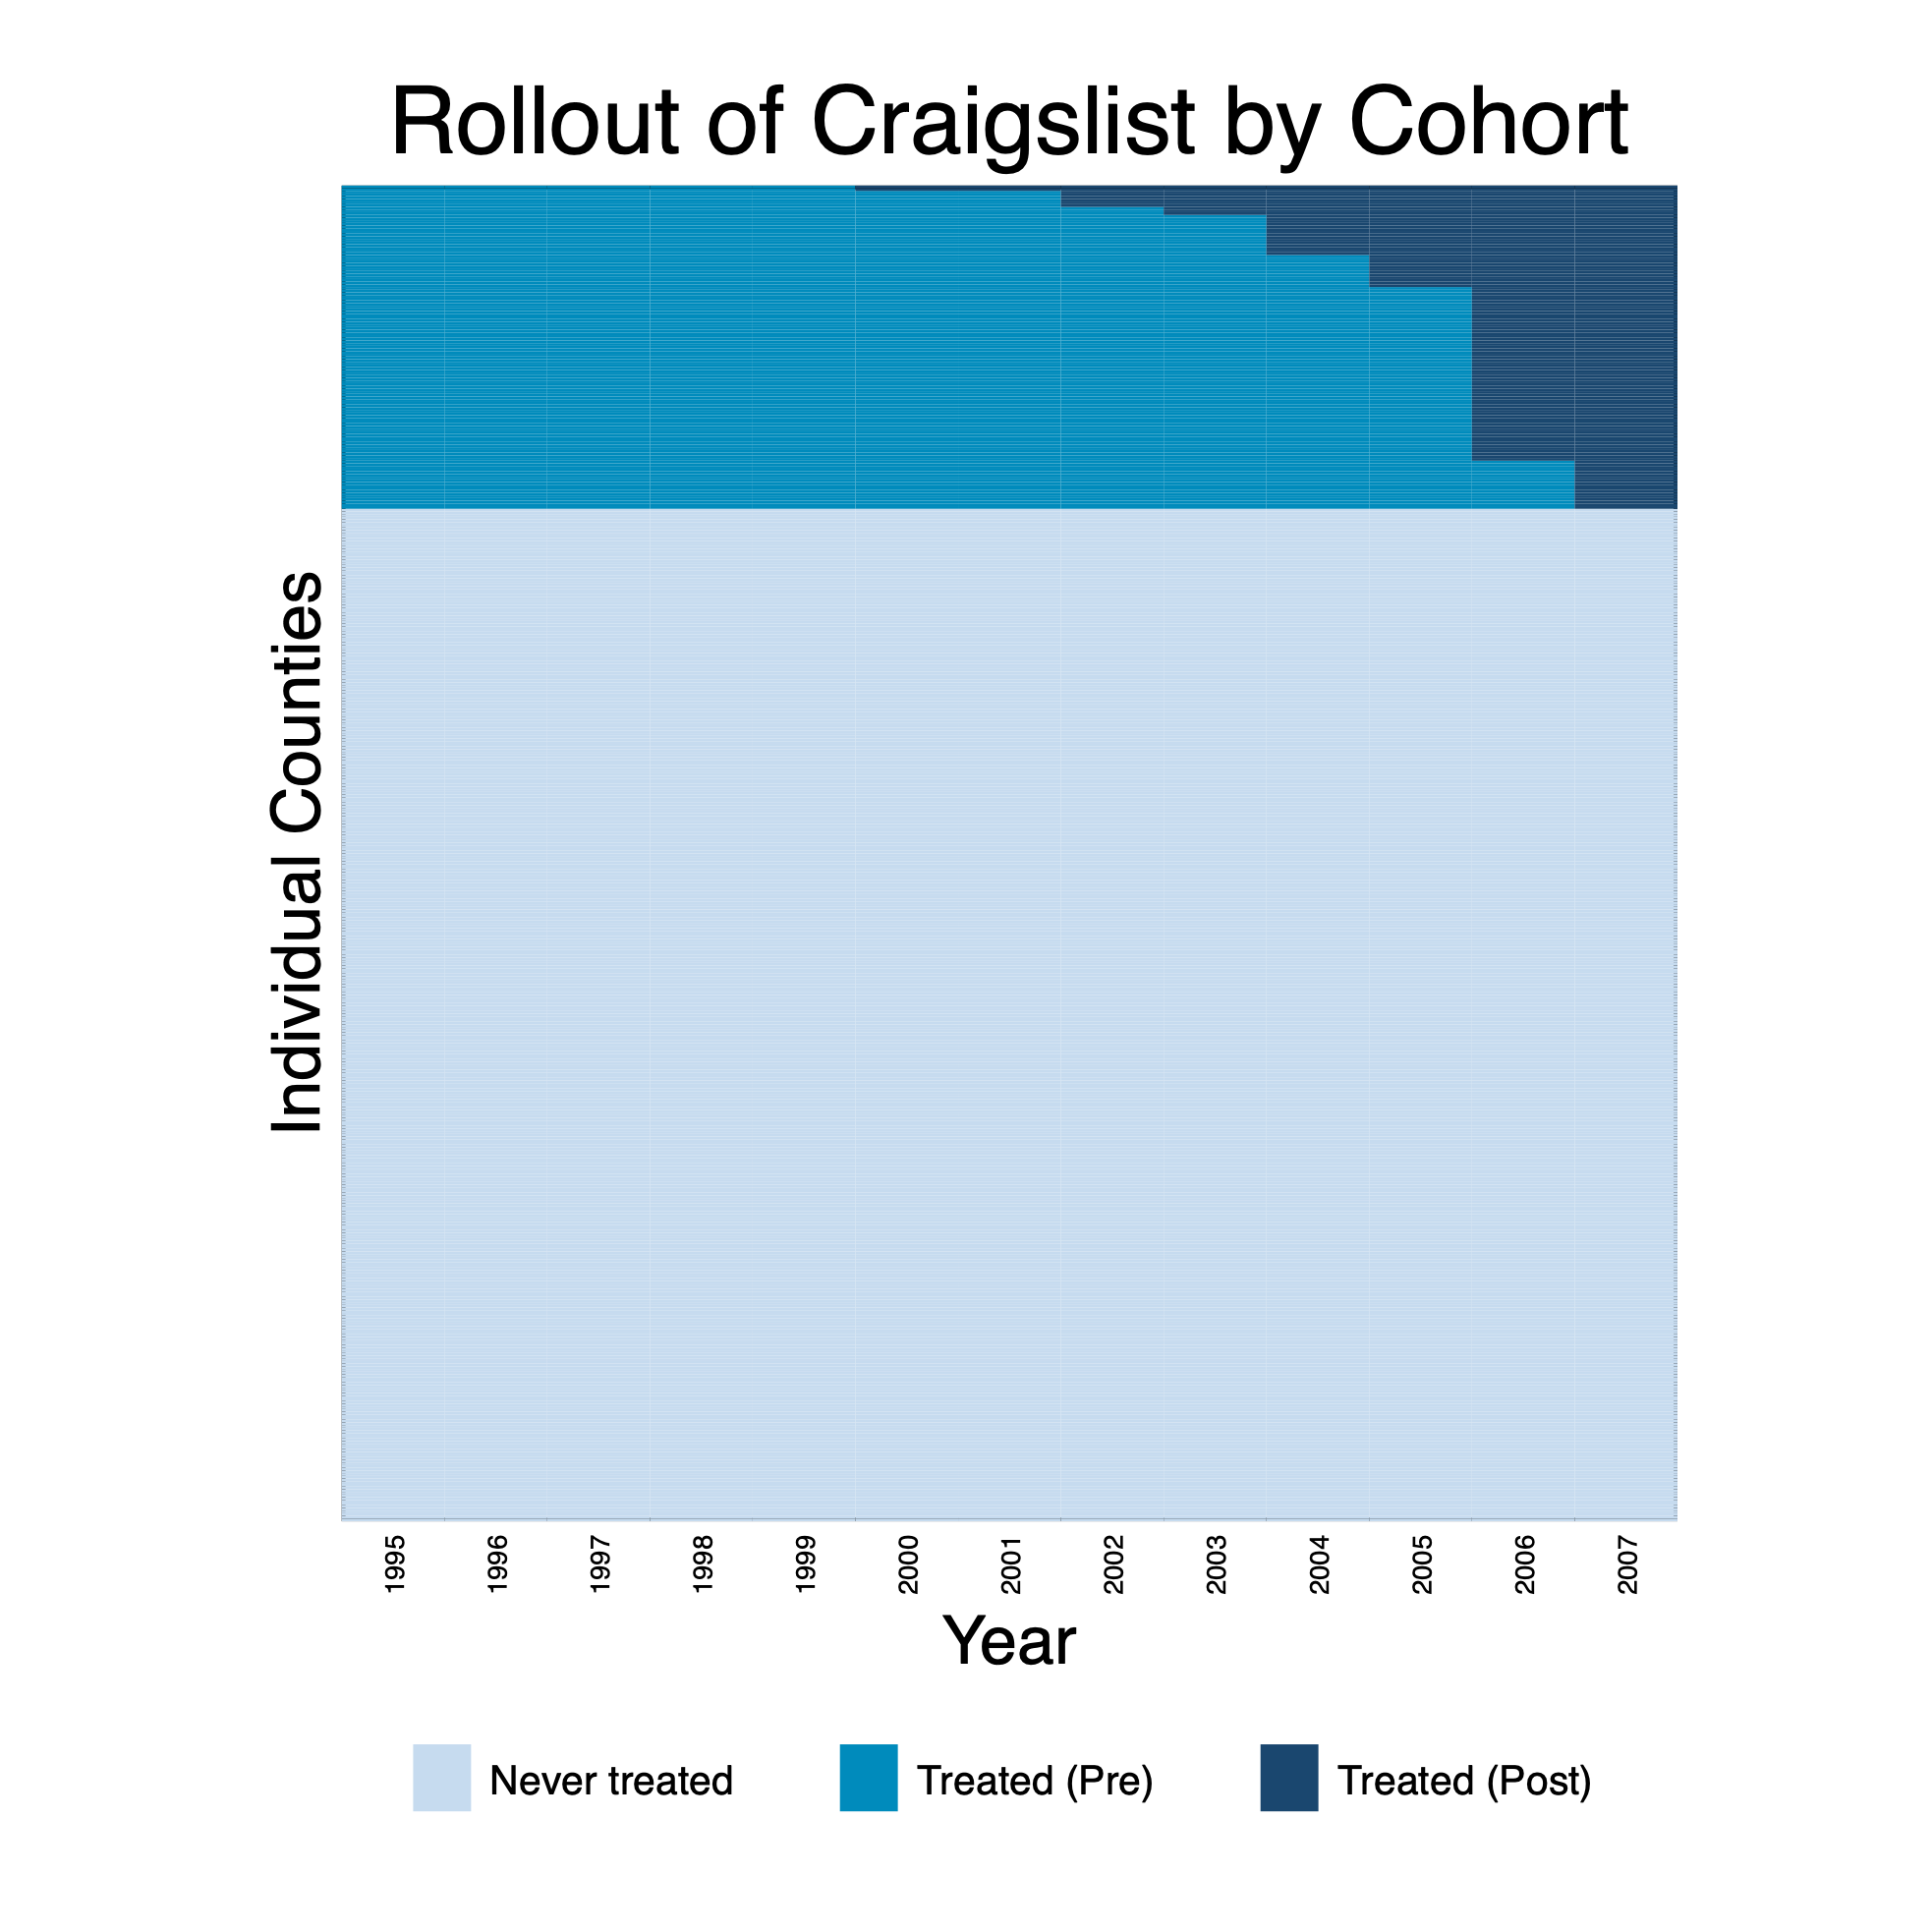
\includegraphics[width=\linewidth, height=0.8\textheight, keepaspectratio]{./lecture_includes/rollout.png}
    \caption{Rollout of Craigslist across US counties.}
\end{figure}

\end{frame}


\begin{frame}{Diff-in-diff checklist: Step 3}

\begin{enumerate}
\item[3. ] Validity of Unconditional Parallel Trends Assumption

    \begin{itemize}
        \item \textbf{Covariate Selection:} Choose covariates predictive of missing potential outcome based on common sense, literature, and expertise.
        \item \textbf{Split-Sample Validation:} Use untreated outcomes with methods like Lasso to identify covariates if unsure.
        \item \textbf{Balance Check:} Check covariate balance using normalized differences.
        \item \textbf{Adjust Imbalanced Covariates:} Adjust if covariates are predictive of potential outcomes $[Y^0|D=1, Post]$.
    \end{itemize}
\end{enumerate}
\end{frame}

\begin{frame}{Rural vs Urban counties}

\begin{itemize}
\item We have a 9-digit ordinal score measuring how urbanized the county is called RUCC
\item Counties that never got a Craigslist were more rural
\item We therefore had originally wanted to use the 2008-2010 and other not-yet-treated counties as comparisons
\item I'll plot rather than show the normalized difference for illustrative purposes
\end{itemize}
\end{frame}

\begin{frame}{Plotting covariate imbalance}

\begin{figure}[ht]
    \centering
    \includegraphics[width=\linewidth, height=0.8\textheight, keepaspectratio]{./lecture_includes/pretty_rucc}
\end{figure}

\end{frame}



\begin{frame}{Comment}

\begin{itemize}

\item Urban counties have different compositions by race, age, sex ratios, education shares, income all of which are \emph{highly} predictive of untreated birth rate trends
\item And even the 2008-2010 counties, despite our original hope, are very rural -- just as rural even
\item So we will run it both ways -- we will run it without controls and then with a single covariate (RUCC)

\end{itemize}

\end{frame}


\begin{frame}{Diff-in-diff Checklist: Step 4}
\begin{enumerate}
\item[4. ] Check Overlap
    \begin{itemize}
        \item \textbf{Overlap Check:} Ensure sufficient overlap in propensity scores.
        \item \textbf{Adjustment for Lack of Overlap:} If lacking, consider a regression adjustment like BJS.
        \item We have overlap since the RUCC code has only 9 values so I'll skip this, but you'll want to check using a propensity score if you have continuous or several covariates
    \end{itemize}
   \end{enumerate}
\end{frame}




\begin{frame}{Diff-in-diff Checklist: Step 5}
\begin{enumerate}
\item[5. ] Plot Average Outcomes Across Cohorts
    \begin{itemize}
        \item Visualize the evolution of average outcomes across cohorts.
    \end{itemize}
   \end{enumerate}
\end{frame}



\begin{frame}{Plotting Outcomes Across Cohorts}

\begin{figure}[ht]
    \centering
    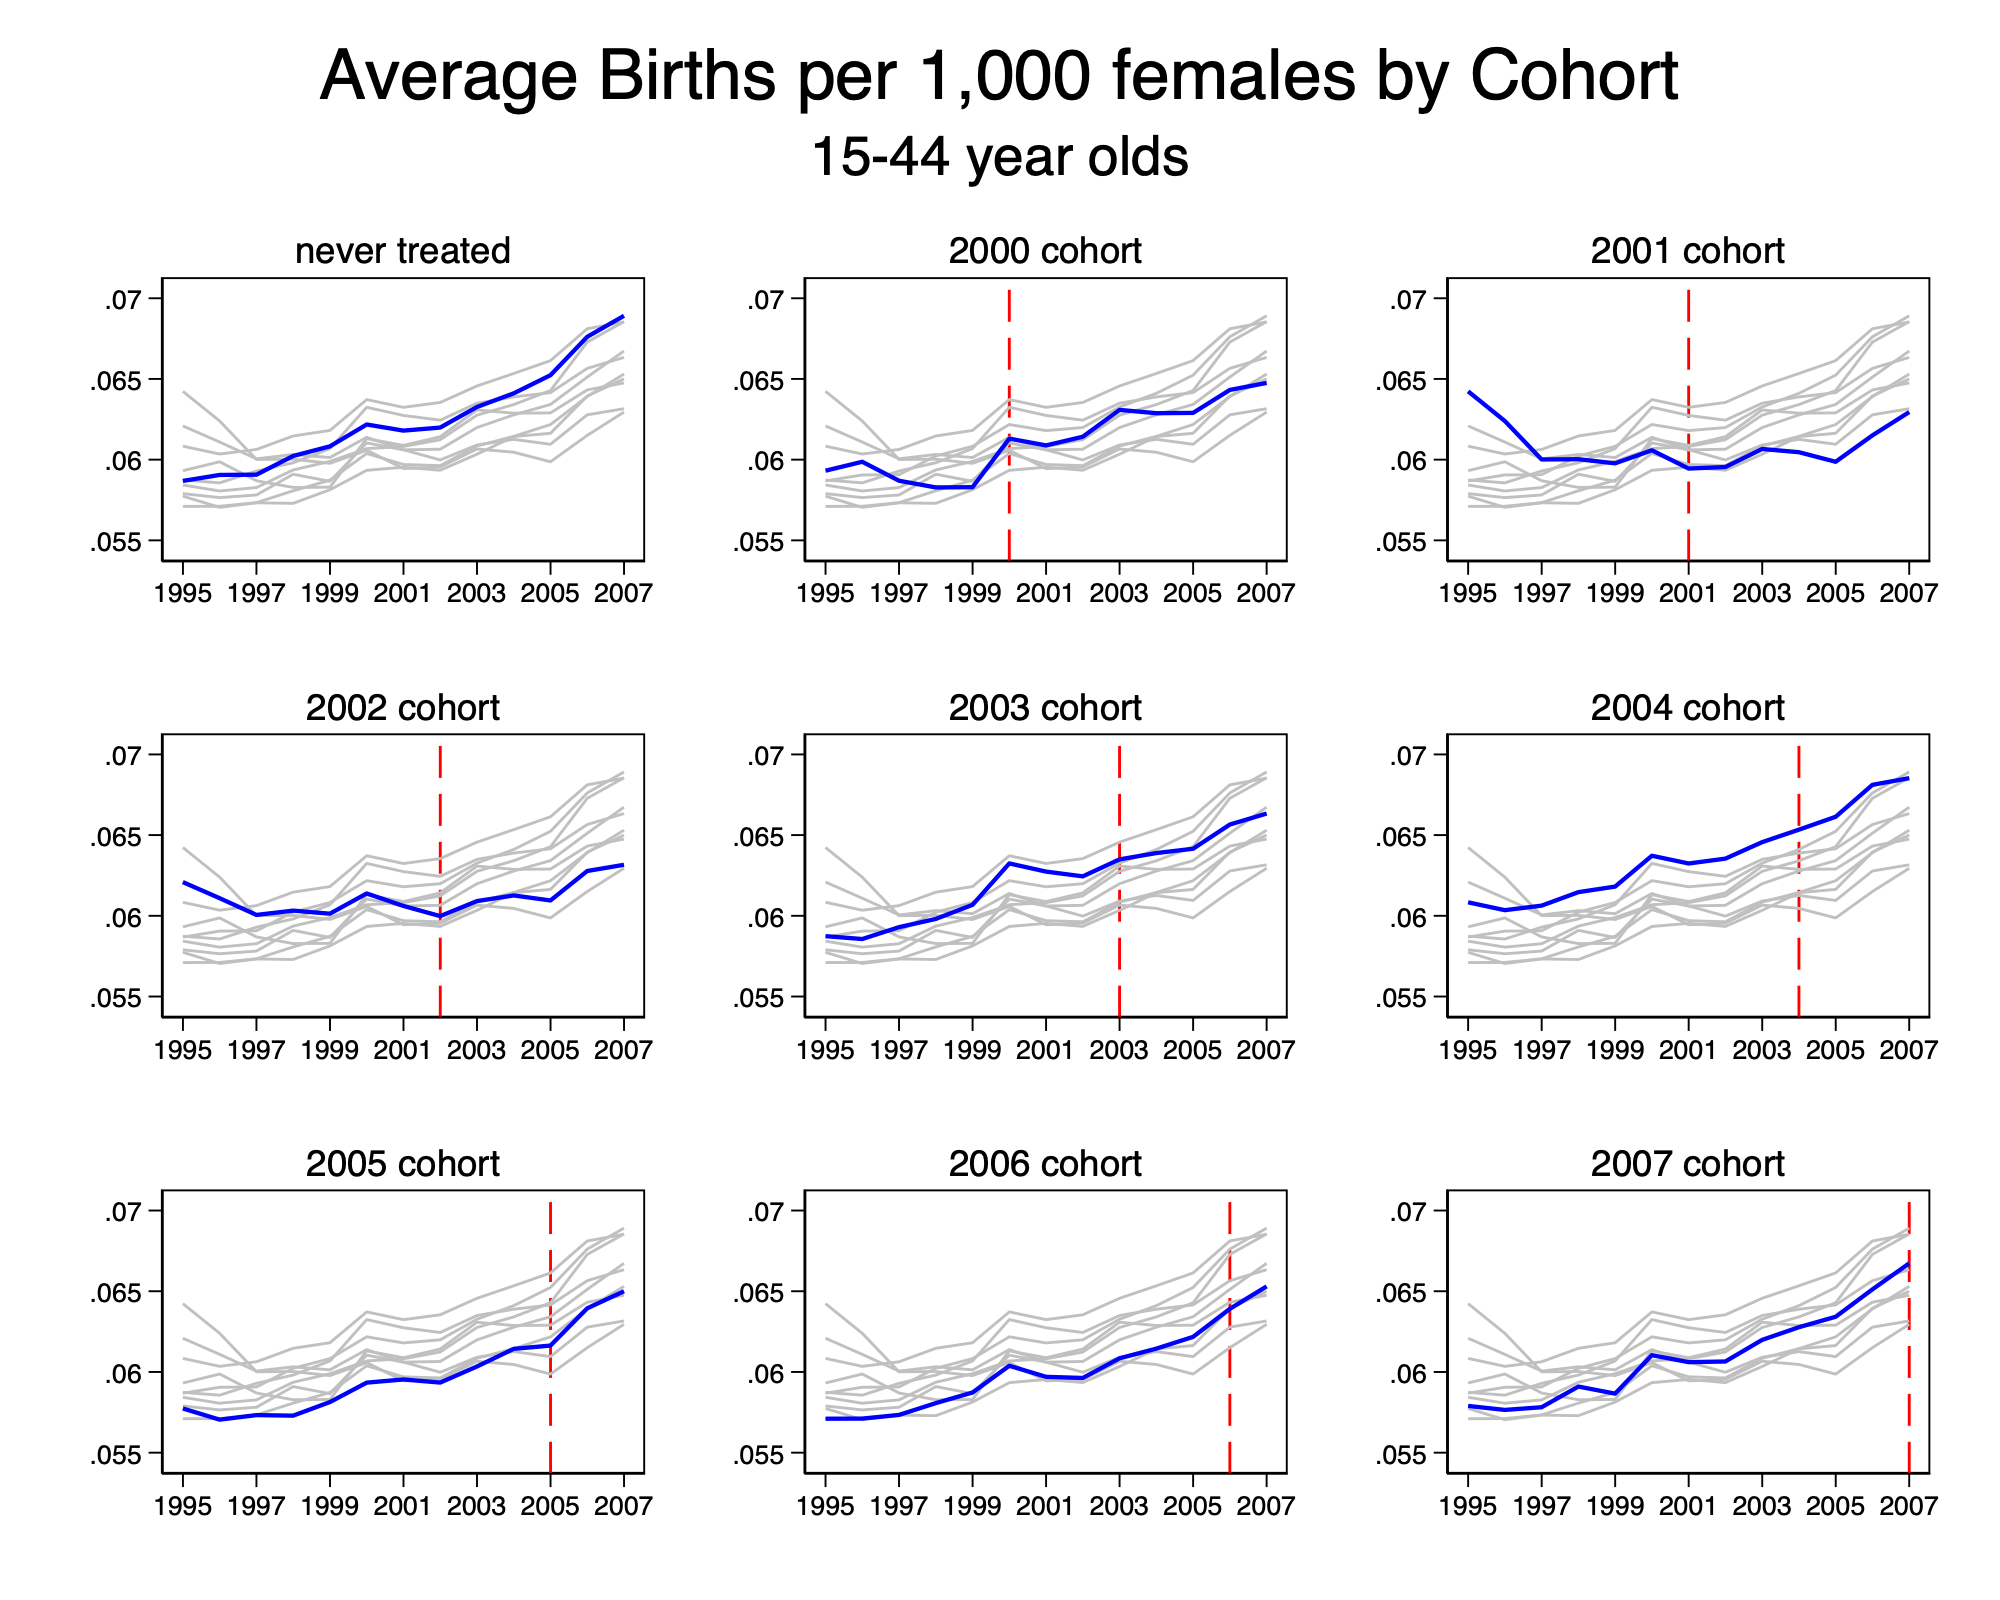
\includegraphics[width=\linewidth, height=0.8\textheight, keepaspectratio]{./lecture_includes/pretty_outcomes.png}
\end{figure}

\end{frame}








\begin{frame}{Diff-in-diff checklist: Step 5}
\begin{enumerate}
\item[5. ]Estimator Selection and Assumptions
    \begin{itemize}
        \item \textbf{Estimator Choice:} Choose an estimator based on comfort and assumptions.
        \item \textbf{Robust Method:} Use robust methods like CS, SA, dCDH, or BJS if agnostic to heterogeneous effects.
        \item \textbf{Event study:} Estimate simple averages as well as event studies 
        		\begin{itemize}
		\item \textcolor{red}{Use long-differences with \texttt{long2} or universal base}
		\end{itemize}
        \item \textbf{Cluster standard errors:} Report with clustering at the aggregate level of treatment.
    \end{itemize}
\end{enumerate}
\end{frame}



\begin{frame}{Short-gaps no controls}

\begin{figure}[ht]
    \centering
    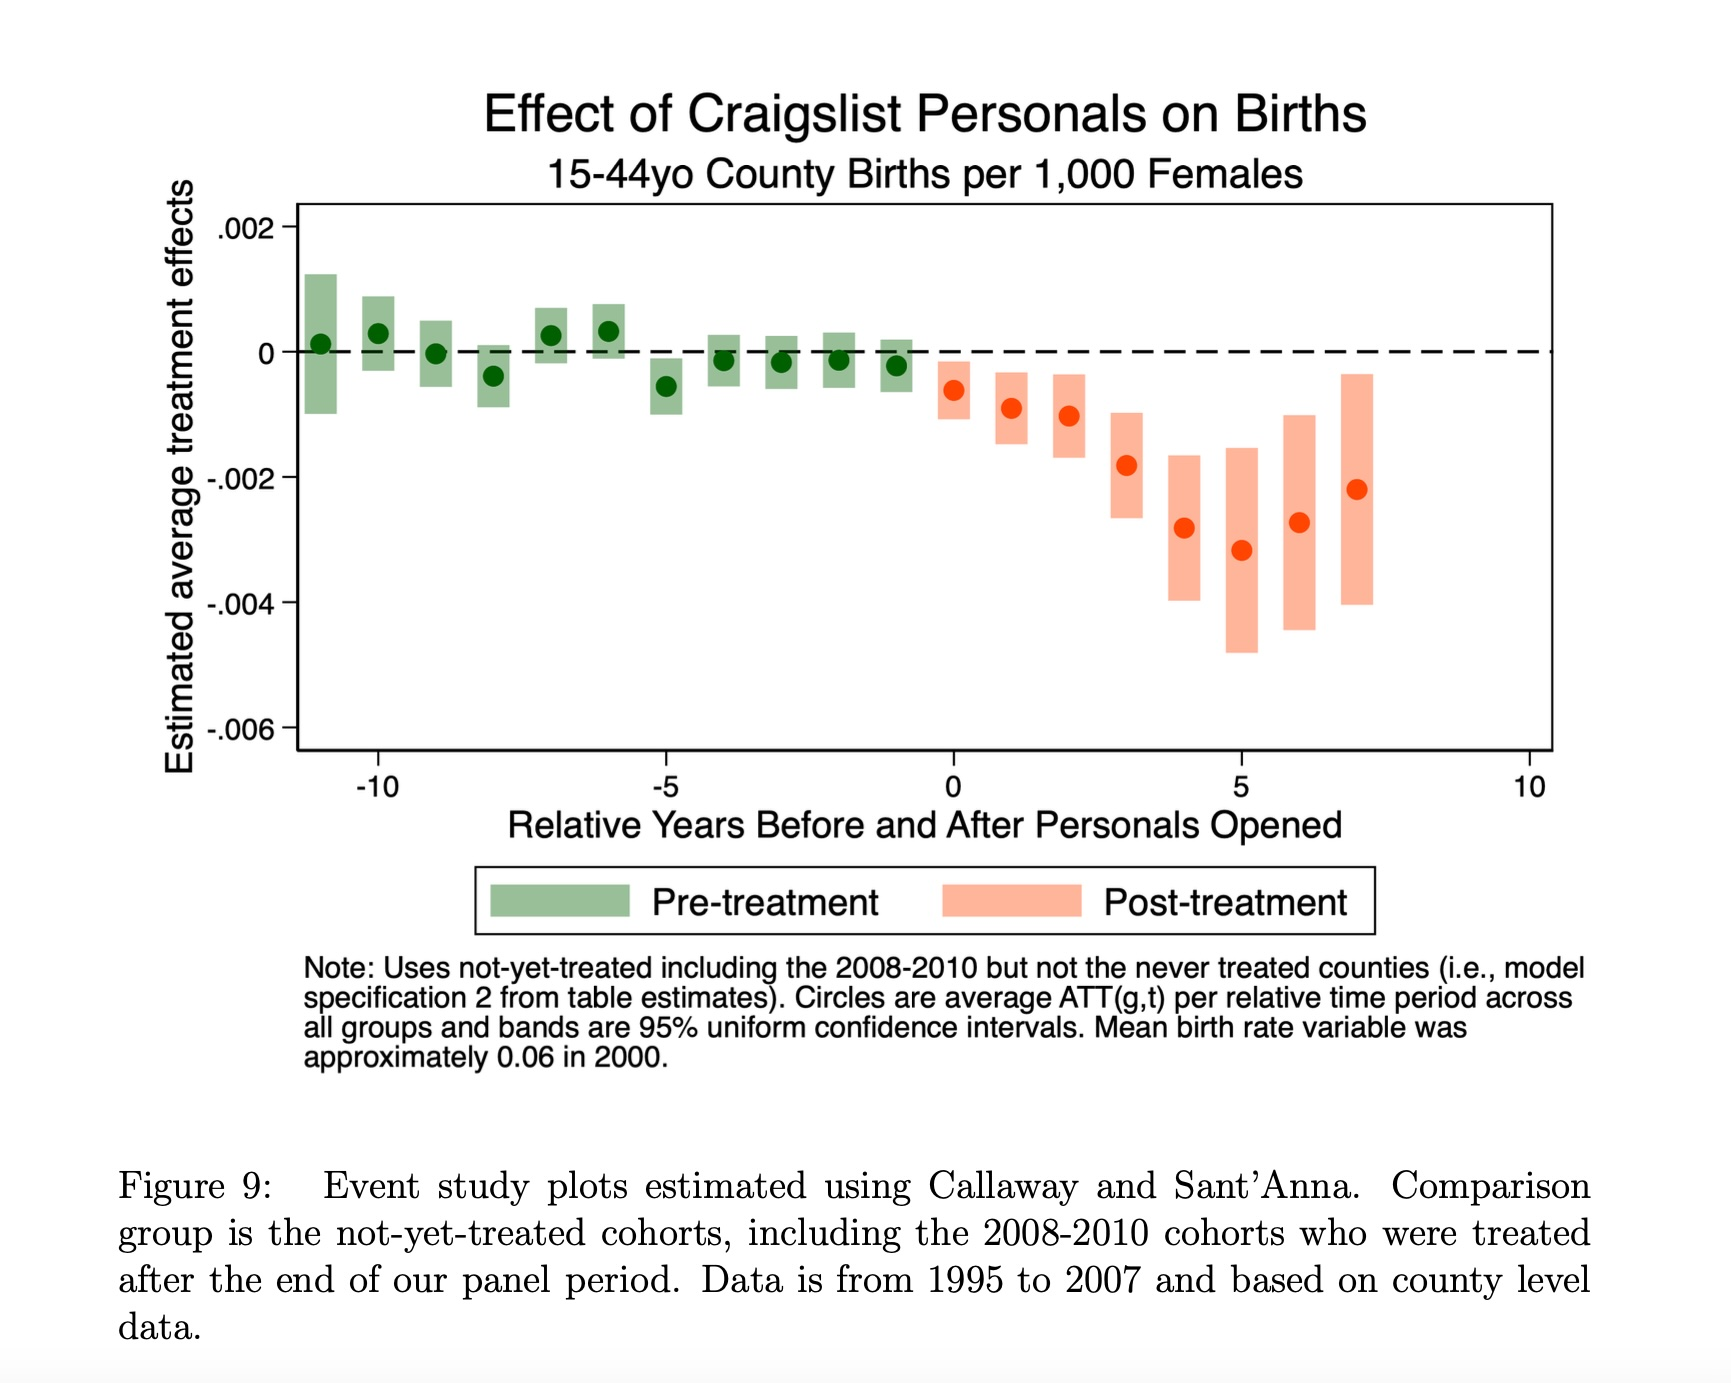
\includegraphics[width=\linewidth, height=0.8\textheight, keepaspectratio]{./lecture_includes/es_births_shortgapNC}
\end{figure}

\end{frame}

\begin{frame}{Long differences no controls}

\begin{figure}[ht]
    \centering
    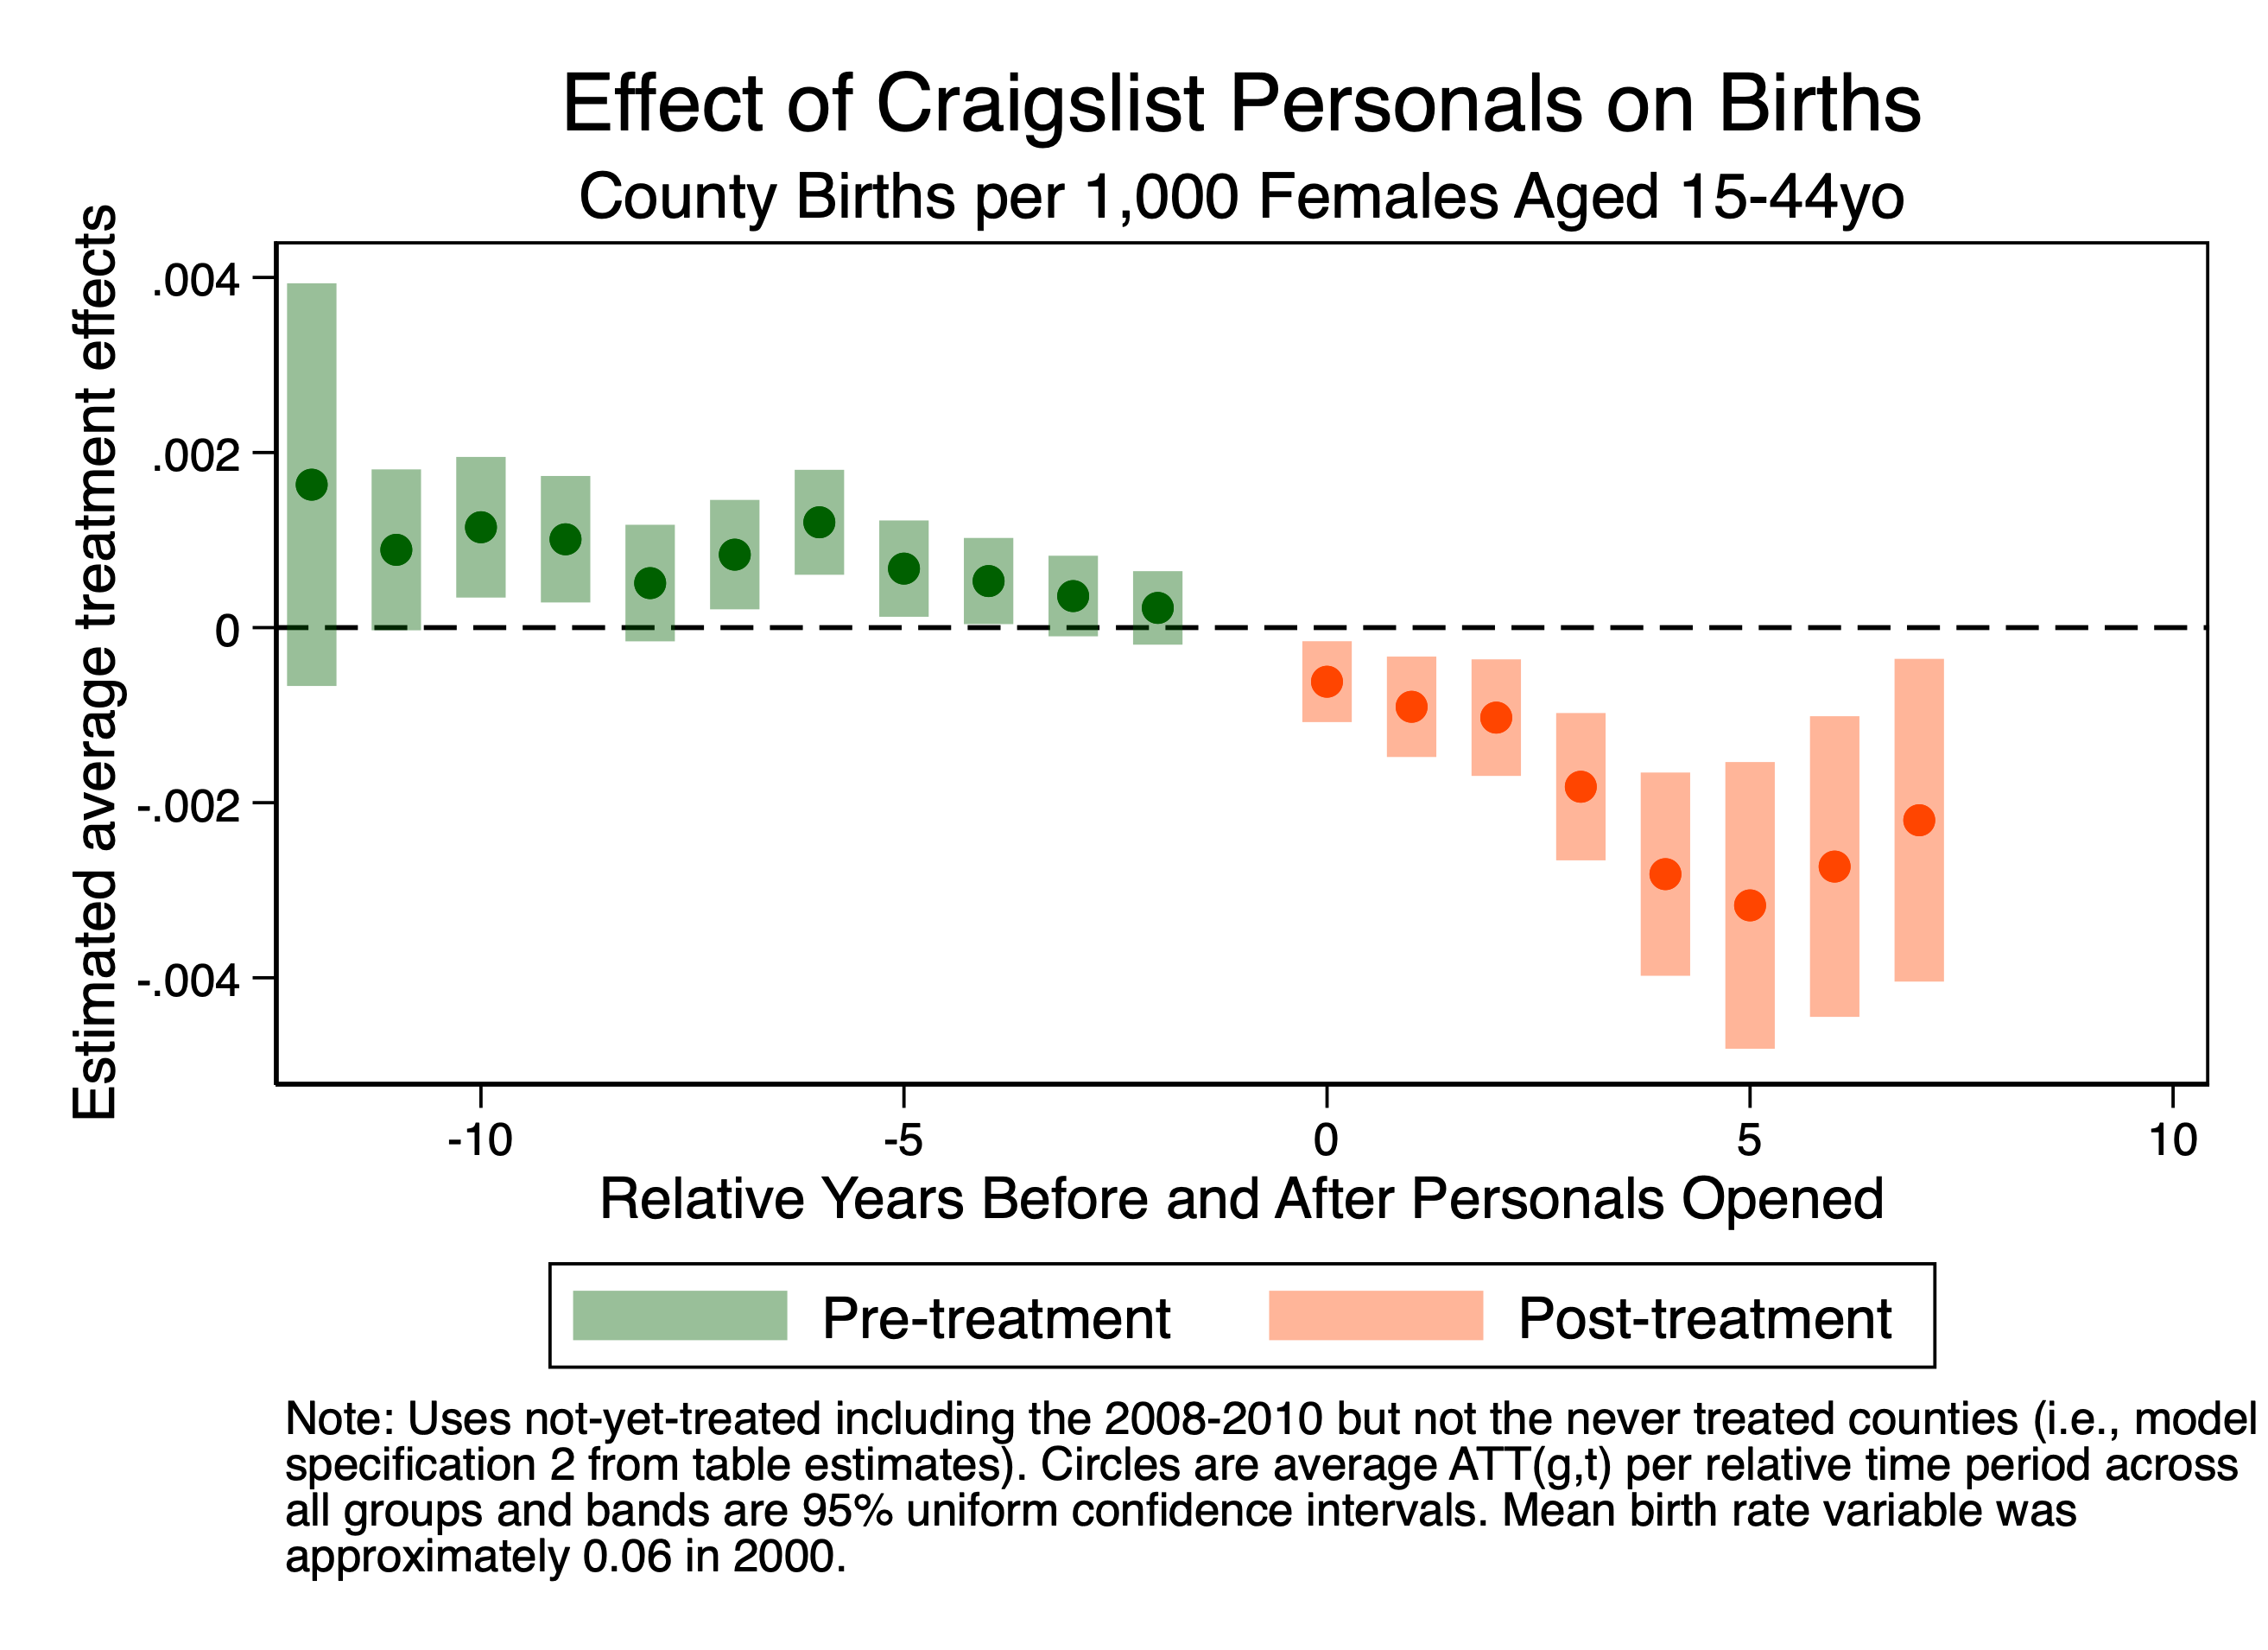
\includegraphics[width=\linewidth, height=0.8\textheight, keepaspectratio]{./lecture_includes/es_births2.png}
\end{figure}

\end{frame}

\begin{frame}{Long differences without and with RUCC control (!)}

\begin{figure}[ht]
    \centering
    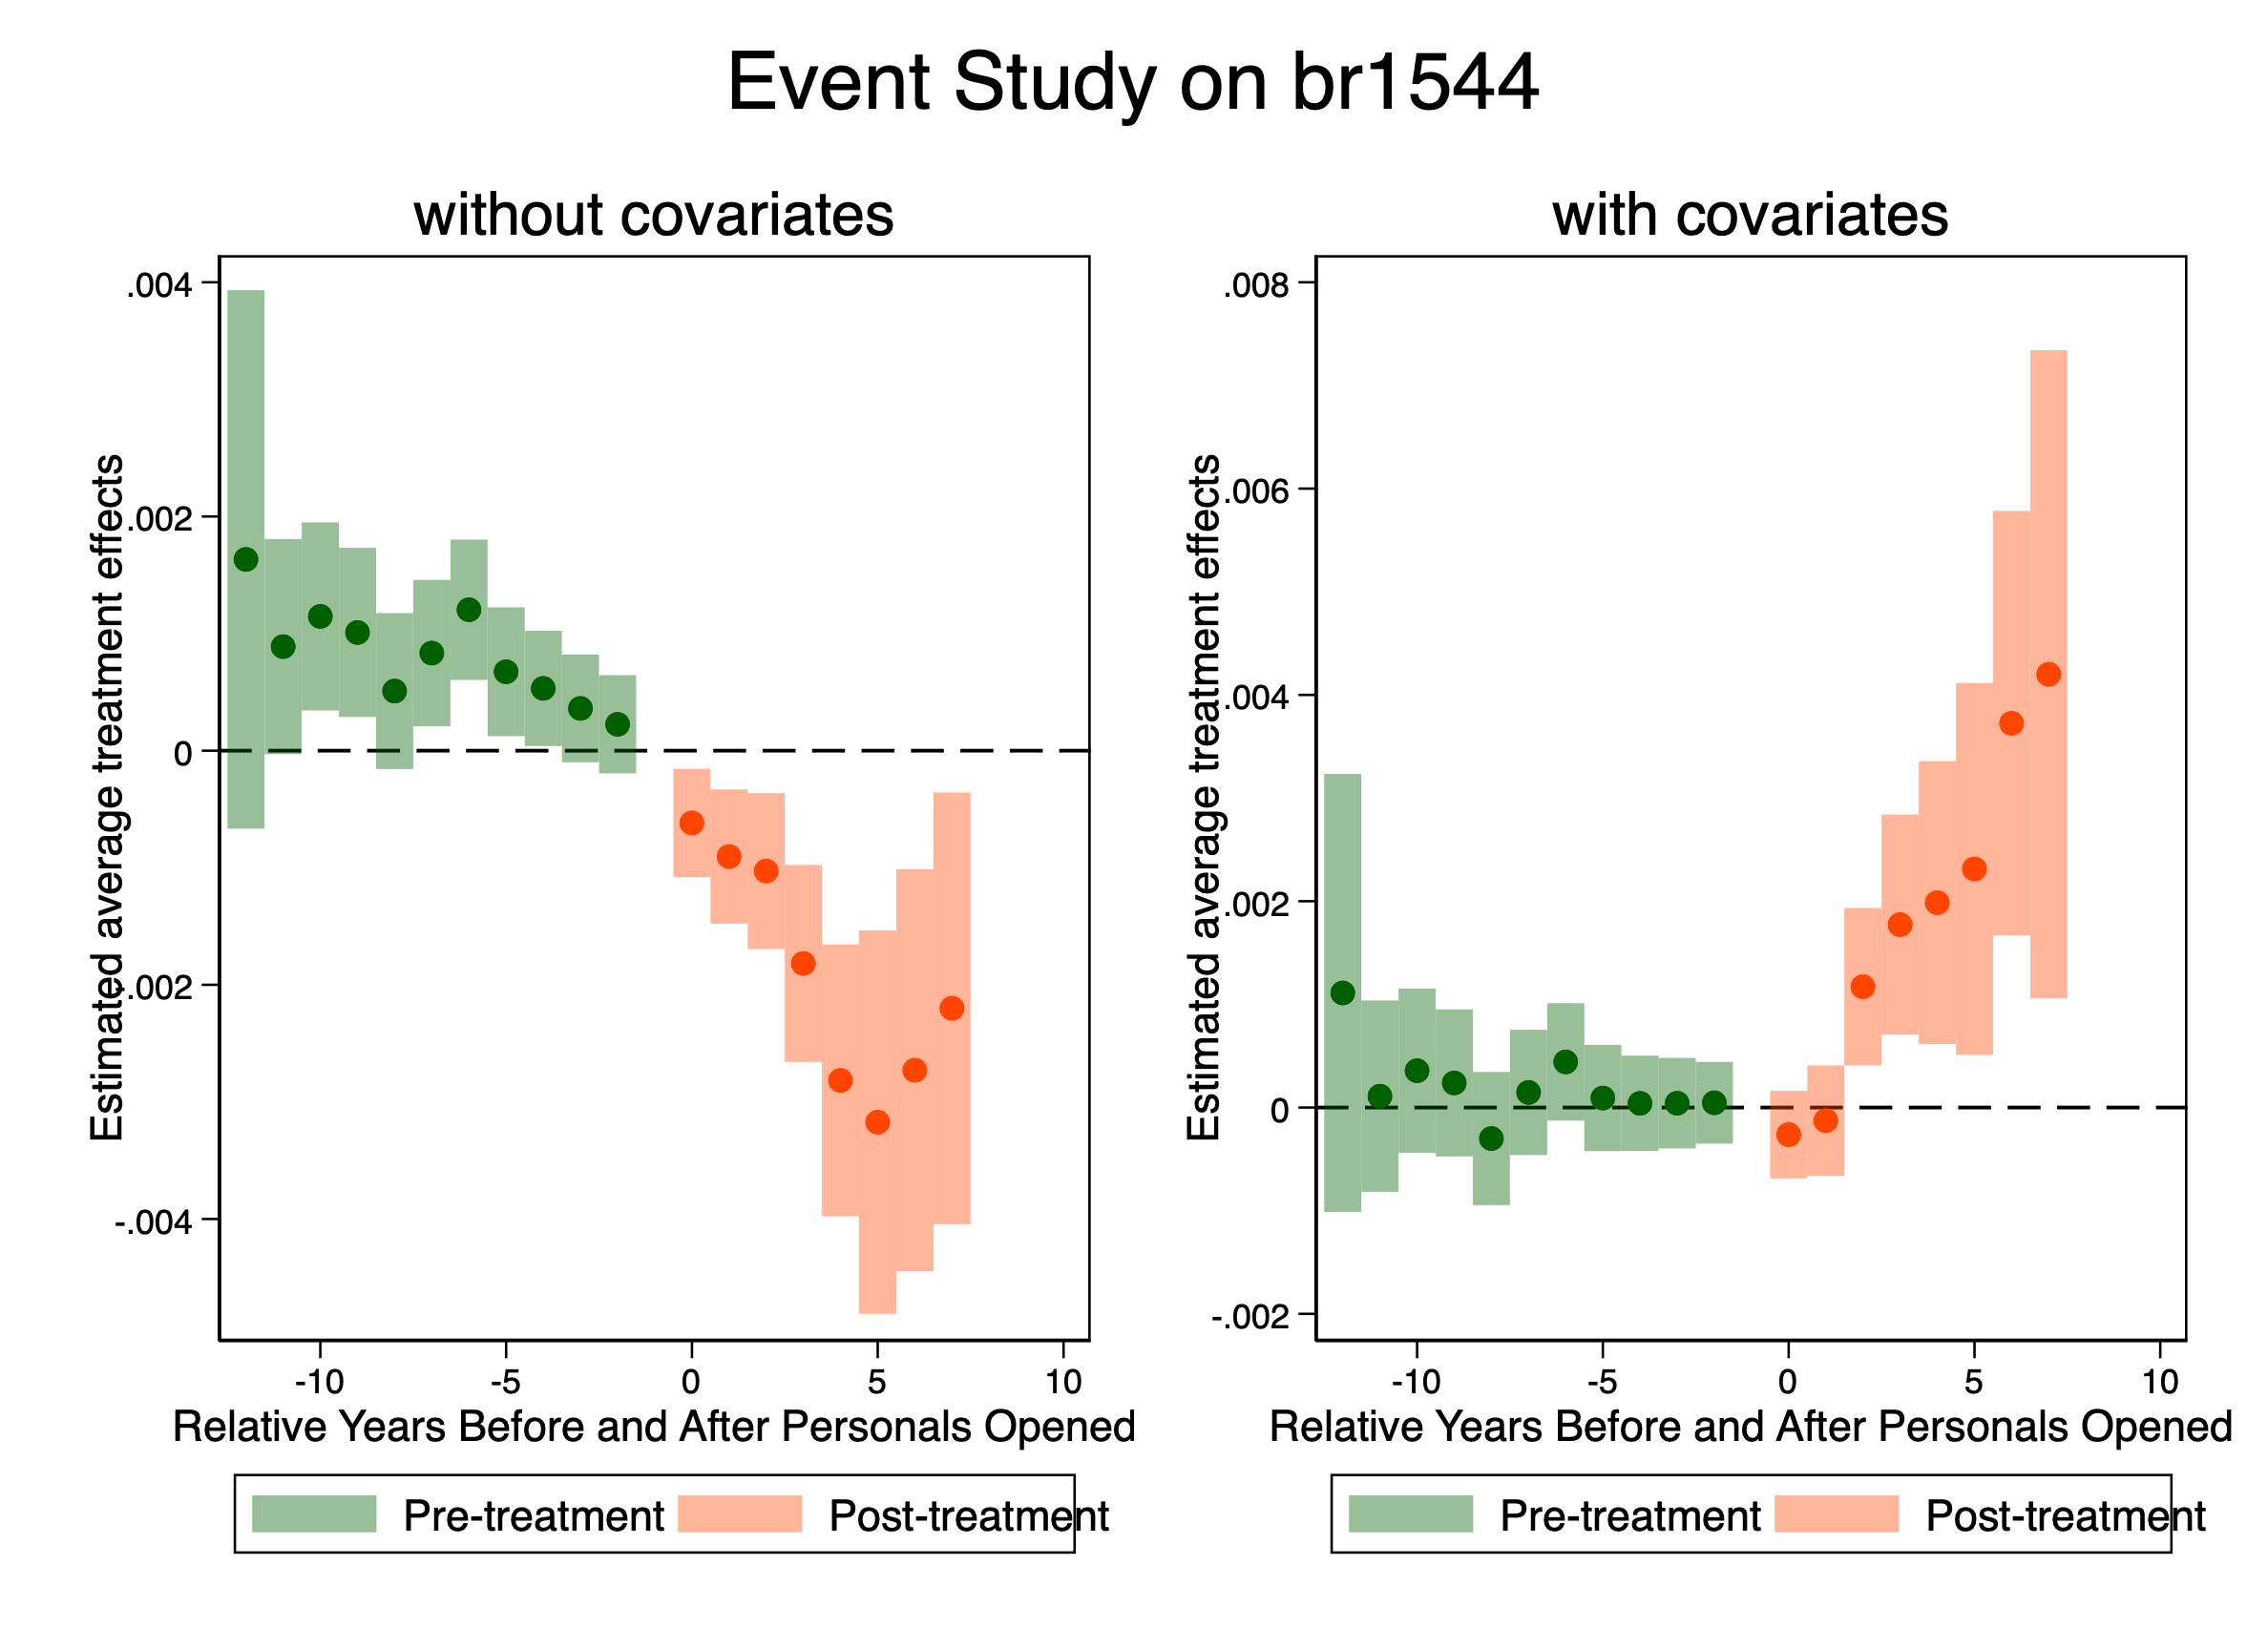
\includegraphics[width=\linewidth, height=0.8\textheight, keepaspectratio]{./lecture_includes/es_br1544_combined.png}
\end{figure}

\end{frame}

\begin{frame}{Running it within each RUCC code}

\begin{figure}[ht]
    \centering
    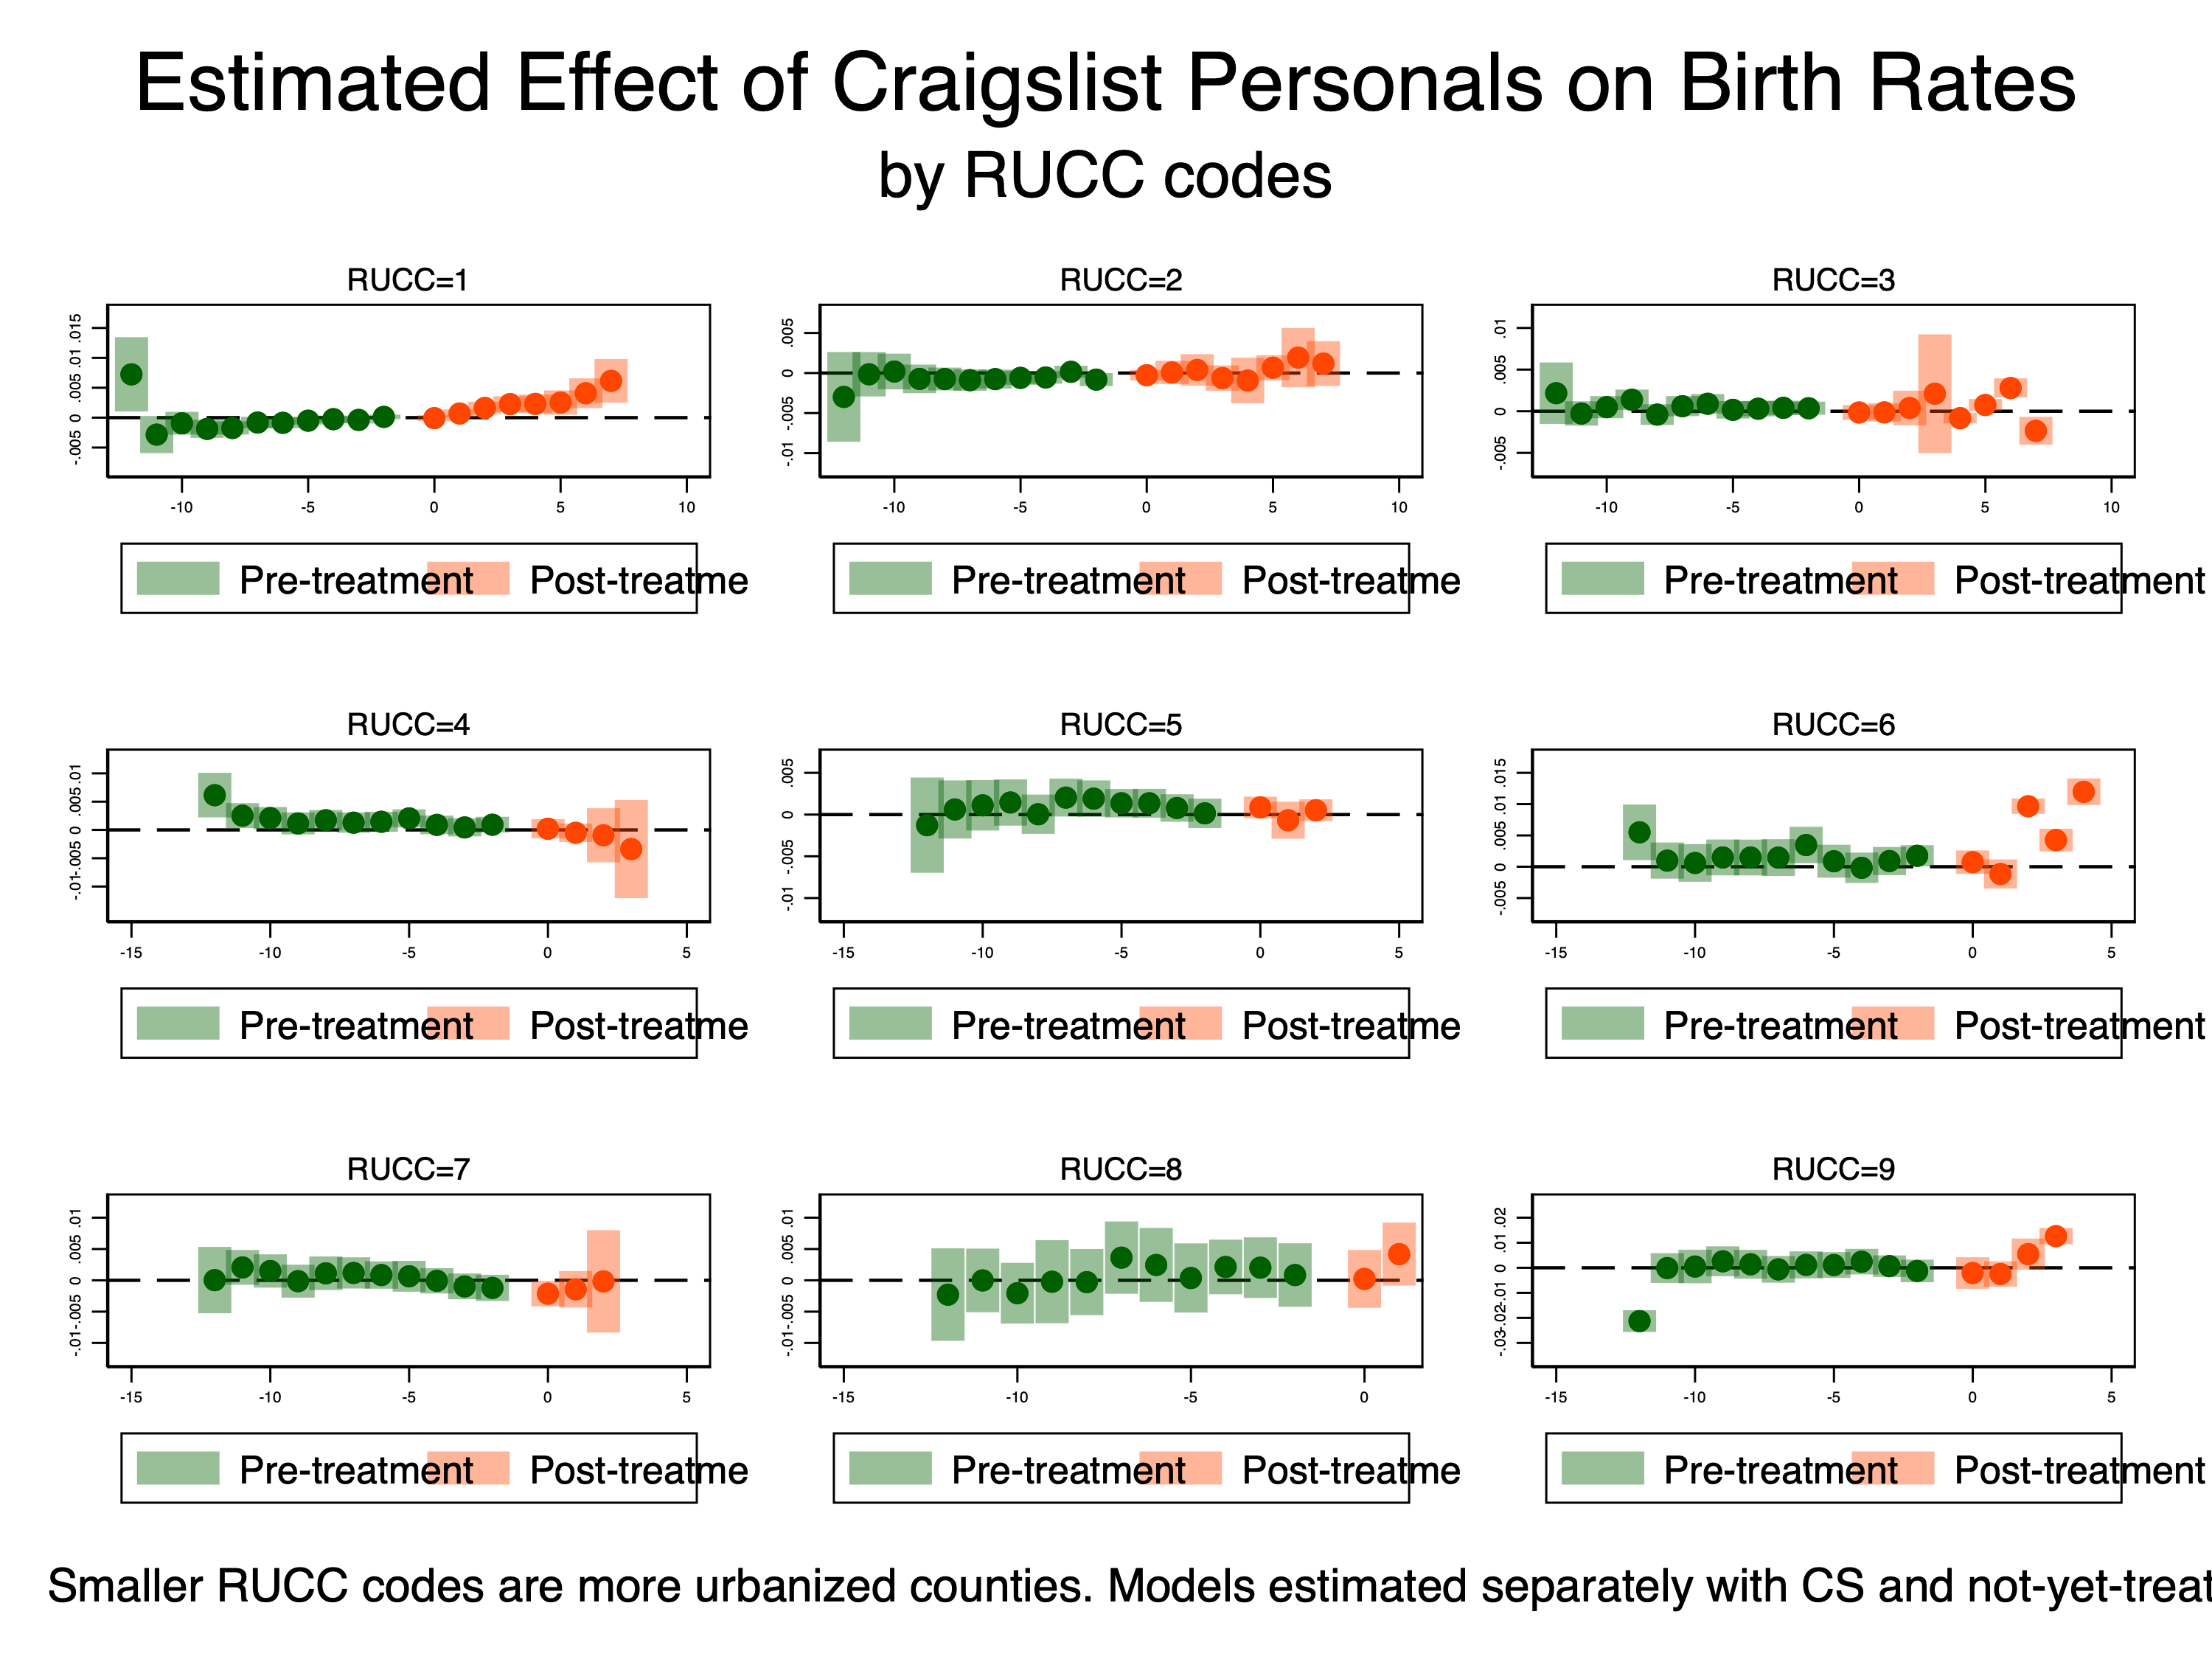
\includegraphics[width=\linewidth, height=0.8\textheight, keepaspectratio]{./lecture_includes/es_br1544_RUCCcombined.png}
\end{figure}

\end{frame}





\begin{frame}{Diff-in-diff checklist: Step 6}
\begin{enumerate}
\item[6. ] Sensitivity Analysis for Parallel Trends Violations
    \begin{itemize}
        \item \textbf{Consider Sensitivity Analysis:} Use tools like \texttt{honestdid} for PT violations.
    \end{itemize}
\end{enumerate}
\end{frame}



\begin{frame}{Diff-in-Diff Checklist: Step 7}
\begin{enumerate}
    \item[7.] Throw in the towel
    \begin{itemize}
        \item You may have to concede that for any number of reasons, parallel trends with or without covariates is implausible — it happens.
        \item Consider then some alternatives:
        \begin{itemize}
            \item \textbf{Panel Method:} If imbalance or PT assumptions fail, consider matrix completion or nuclear norm regularization.
            \item \textbf{Cross-Section:} Cross-sectional unconfoundedness may also be appropriate.
        \end{itemize}
        \item Don’t force it — diff-in-diff doesn't make estimates causal; parallel trends makes diff-in-diff causal.
    \end{itemize}
\end{enumerate}
\end{frame}


\section{Concluding Remarks}

\begin{frame}{Concluding remarks on DD}

\begin{itemize} 
\item You're probably going to write a paper using DiD at least once in your life, but probably more
\item Even if you don't, you're going to read a lot of papers using DiD, referee them, or advise students using them
\item It's in your best interest to make the fixed cost investment in the new econometrics of DiD because the old methods are mostly harmful
\item Good news is we are at the conclusion of this wave of papers, software is now widely available, solutions tend to have common features, and overall presentations (static and dynamic) aren't all that different
\item Lots of surveys have been written (Roth, et al. 2023; our new JEL) and you'll have the slides and recordings here
\end{itemize}

\end{frame}

\begin{frame}{Concluding remarks}

\begin{itemize}
\item Stronger assumptions needed to include covariates, and bias can be large
\item But you need the correct covariates, and I suggested using sample splitting for selection and LASSO to identify relevant covariates that affect \textbf{untreated potential outcomes}
\item Don't control for covariates that could be affected by the outcome 
\end{itemize}

\end{frame}

\begin{frame}{Concluding remarks}

\begin{itemize}
\item Main problem in differential timing is heterogeneity and the use of already-treated units as controls
\item Differential timing and lacking a priori theory, you \emph{should} avoid the canonical TWFE specification  
\item With heterogeneity, canonical TWFE is biased, signs can flip, weights can be negative, etc etc.
\item Robust DiD methods do not place restrictions on treatment effect heterogeneity, but cannot solve everything
\item But when you lose parallel trends, you're probably going in the direction of need a new design
\end{itemize}

\end{frame}

\begin{frame}{Concluding remarks}

\begin{itemize}
\item Devote time to designing your diff-in-diff -- you'll thank yourself as it keeps you honest and helps identify problems before having peeked at the outcomes
\item Much harder psychologically to pull back when you've become invested in a story, so do not go to the outcomes until you've pre-registered your study to some degree (even if not formally)
\end{itemize}

\end{frame}

\begin{frame}{Conclusion}

\begin{itemize}
\item Thank you for coming to the workshop
\item I hope that this was valuable for you
\item We will be doing this until demand drops off, so keep your eyes peeled
\end{itemize}

\end{frame}








\end{document}
